\documentclass[a4paper, 12pt]{article}
% math symbols
\usepackage{amssymb}
\usepackage{amsmath}
\usepackage{mathrsfs}
\usepackage{physsummer}


\usepackage{enumitem}
\usepackage[margin = 2cm]{geometry}

\tolerance = 1000
\emergencystretch = 0.74cm



\pagestyle{empty}
\parindent = 0mm

\setphysstyle{ФМЛ 239, 9 класс}{Занятие 4}{17 октября 2015}

\begin{document}

\begin{center}
  \LARGE{\textbf{Стандартные задачи} }
\end{center}

\Large

\task{ Скоростной поезд на испытаниях движется по окружности радиусом
  $R=10$ км. Через 100 с после начала движения скорость поезда,
  равномерно возрастая, достигает величины 360 км/ч. Найдите
  зависимость полного ускорения поезда от времени $t$. }
% Манида, 168

\task{ Диск радиуса $R$ помещён между двумя параллельными
  рейками. Рейки движутся со скоростями $v_1$ и $v_2$. Определить
  угловую скорость вращения диска и скорость его
  центра. Проскальзывание отсутствует. }
% Квант-1972-09, Асламазов, стр. 57

\taskpic{ Точка движется вдоль оси $x$. График зависимости скорости от
  координаты представлен на рисунке~---~он представляет собой дугу
  окружности. Найдите время перемещения от $0$ до $x_0$ и ускорение
  при приближении к точке $x_0$. }
{
  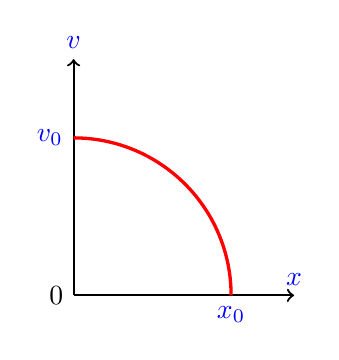
\begin{tikzpicture}
    \draw[thick,->] (0,0) node[left] {0} -- (2.8,0) node[above,blue] {$x$};
    \draw[thick,->] (0,0) -- (0,3) node[above,blue] {$v$};
    \draw[very thick, red] (0,2) node[left,blue] {$v_0$} arc
    (90:0:2cm) node[below,blue] {$x_0$}; 
  \end{tikzpicture}
}
% Зильберман, 1.34

\begin{center}
  \LARGE{\textbf{Сложная задача} }
\end{center}

\task{ Компакт-диск вращается со скоростью 78 оборотов в минуту. По
  нему ползёт жук, его скорость относительно пластинки 1 см/c, он
  движется по радиусу к центру пластинки. Найти его ускорение в тот
  момент, когда расстояние до центра составляет 10 см. }
% Зильберман, 1.33

\begin{center}
  \LARGE{\textbf{Фольклор} }
\end{center}

\task{ В вершинах квадрата со стороной $a$ сидят четыре жука. В
  некоторый момент они начинают двигаться с постоянной по модулю
  скоростью $v$, причём первый жук движется в направлении второго,
  второй --- в направлении третьего, третий --- в направлении
  четвёртого, а четвёртый --- в направлении первого. Через какое время
  они встретятся? }

\end{document}


%%% Local Variables: 
%%% mode: latex
%%% TeX-engine:xetex
%%% TeX-PDF-mode: t
%%% End:
